\chapter{Background}

In this chapter we compare streaming data flow architectures with
traditional, general purpose architectures and we describe the Maxeler
hardware acceleration solution and the MaxCompiler toolchain and API
which represent the target of the MaxC compilation process. We also
look at the LARA language which will be used as part of the design
flow to specify and apply optimization strategies both to the original
source code and to the resulting dataflow design. We also summarize
related work in the area of high level synthesis tools.


\section{Dataflow Computing}

\subsection{Multi-core}

\subsection{GPU}

\subsection{FPGA}

Although general purpose computing devices offer a convenient
programming paradigm, the traditional fetch - decode - execute cycle
is inherently sequential and relies on inefficient access to external
memory. To compensate for this a large area of a modern CPU core is
dedicated to caches, branch prediction units and out-of-order
scheduling and retirement units. This reduces the area of the chip
available for performing useful computation. Furthermore, although
multicore programing is an answer for the processor power wall (which
prevents increases in operating frequency beyond a certain point,
limiting the processing speed of a single core device), there are
classes of algorithms whose performance does not scale linearly with
the number of cores. This is especially true when operating on large
volumes of data with poor spatial locality that do not fit into a
CPU's on-chip cache such as algorithms involving sparse matrix
computations or convolution [@survive1]. Although this model offers
good flexibility when dealing with arbitrary access patterns, it is
not efficient for large volumes of highly regular data.

The dataflow computing paradigm operates differently form the general
purpose computing paradigm (as shown in Figure \ref{fig:cpudfe}),
being designed to be efficient at processing large volumes of data. It
works by creating a streaming dataflow graph of computational nodes,
which operates as a large computational pipeline: input data is
streamed in sequentially through each pipeline stage and output data
is streamed out. This results in a highly pipelined design that can be
statically scheduled achieving throughput rates of one value per cycle
by completely avoiding pipeline hazards. This means that a design
running at a few hundred megahertz can easily outperform a CPU
implementation running at a few gigahertz while being more energy
efficient [@survive2].


\begin{figure}[h] \centering
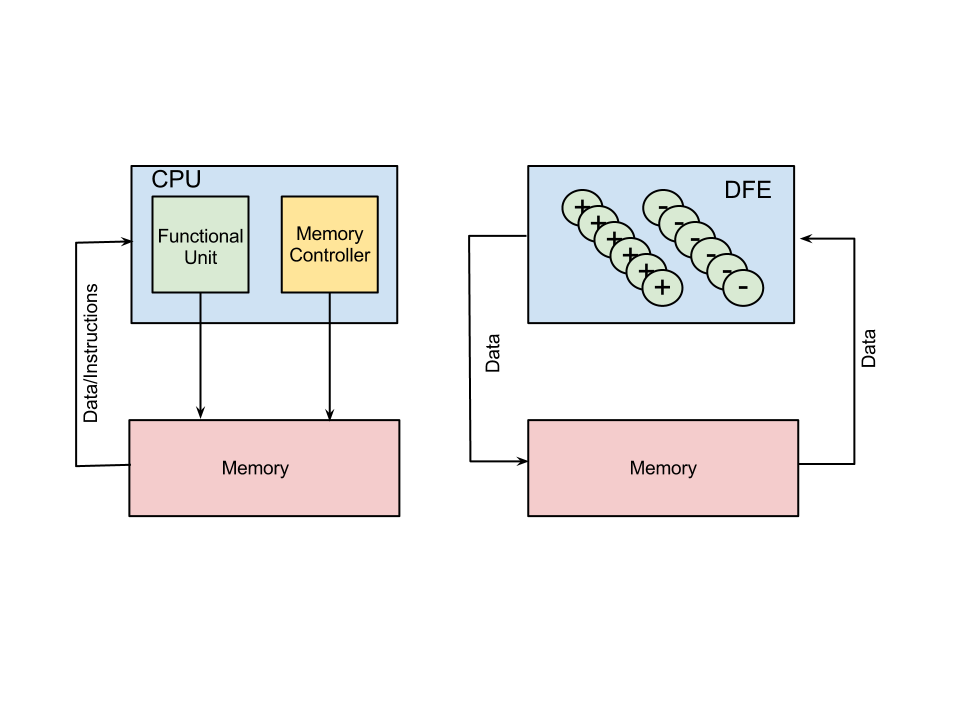
\includegraphics[scale=0.4, trim=0 200 0 150]{figs/cpu-vs-dfe.png}
\caption{Comparison between general purpose CPU architecture and a
streaming Data Flow Engine. In the case of the latter instructions are
not stored in memory but encoded in the dataflow graph. }
\label{fig:cpudfe}
\end{figure}

\section{Maxeler Acceleration Solution}

Maxeler Technologies provides a software and hardware acceleration
solution based on the dataflow computing model. The dataflow design is
created using MaxCompiler [@maxwhite] and implemented on a specialized
hardware platform, built around high-end Field Programmable Gate Array
(FPGA) chips.



FPGAs are logic chips that can be reconfigured in seconds to implement
custom applications. Hence they offer a much shorter time to market
than traditional ASIC\footnote{Application Specific Integrated
  Circuit} based solutions, while still being able to implement custom
logic circuits, making them significantly faster than general purpose
hardware. However, the size of the FPGA chip constrains the design
that can be uploaded onto the chip. FPGAs have a limited number of
each of the following resource types:



\begin{itemize}
\item look-up tables (LUTs) - implement the logical functions performed by the circuit;
\item flip-flops (FFs) - small storage elements;
\item digital signal processors (DSP) - small special purpose arithmetic units;
\item block RAM (BRAM) - larger, on-chip storage elements.
\end{itemize}



The specific data flow engine used for this project is a MAX3424A card
based on a Virtex 6 FPGA chip [@virtex6]. The MAX3 provides 48GB of
on-board DRAM and about 4MB of fast on-chip BRAM are available on the
FPGA chip.

The system is connected to the dataflow engine via PCIe as shown in
Figure \ref{fig:max3}.

\begin{figure}[h]
\centering
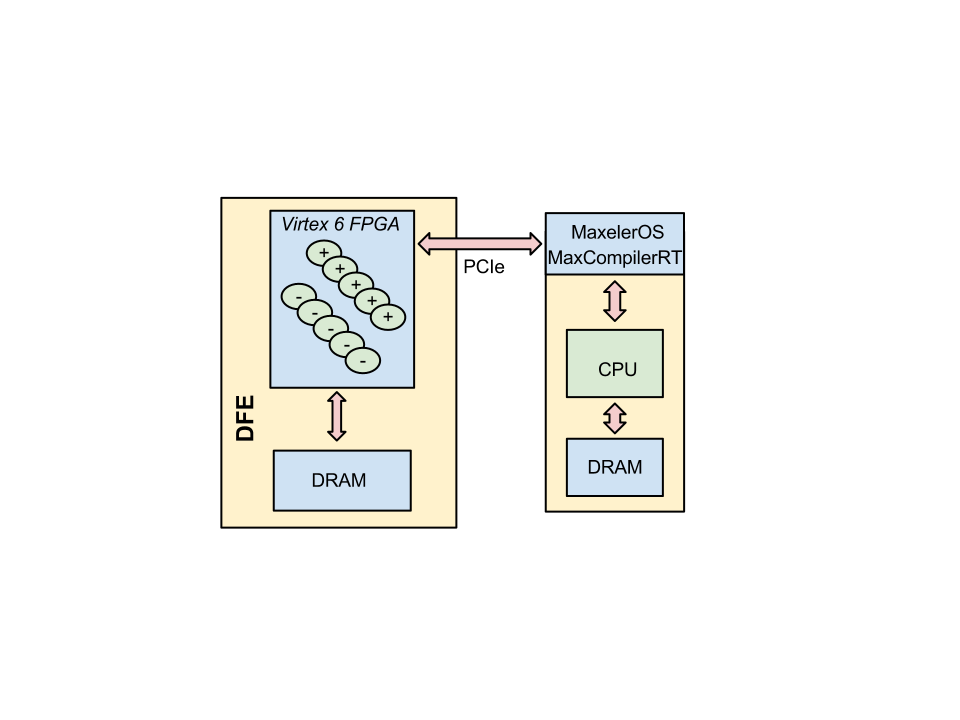
\includegraphics[scale=0.4, trim=0 200 0 200]{figs/max3.png} \caption{
The Maxeler acceleration solution: the DFE is connected to
the host machine via PCIe. The board comprises 48GB of DRAM and a
Virtex 6 FPGA chip. }
\label{fig:max3}
\end{figure}

\subsection{MaxJ}

\subsection{MaxCompiler}

MaxCompiler is a high level compiler targeting the acceleration
platform developed by Maxeler Technologies [@maxwhite]. It provides a
Java based API for specifying hardware designs that are compiled and
uploaded onto the DFE and a C runtime interface (MaxCompilerRT and
MaxelerOS shown in Figure \ref{fig:max3}) for the part of the
application running on the CPU of the host system.

We demonstrate the use of MaxCompiler in accelerating a simple moving
average computation, starting from an original design in C shown in
Listing \ref{MovingAvg-C}. This performs a three point moving average
computation on an input array x, using 2 point averages at boundaries.

\lstset{language=C++, caption={Original three point moving average
computation in C.}, label={MovingAvg-C}}

\begin{lstlisting}

for (int i = 0; i < n; i++ ) {
   sum = x[i], divisor = 1;
   if ( i > 0 )
     sum += x[i - 1], divisor++;
   if (i < n - 1)
     sum += x[i + 1], divisor++;
   y[i] = sum / divisor;
}
\end{lstlisting}



Transforming this code to use the Maxeler acceleration platform
requires us to write three programs.

First we must create a kernel design. This is written in Java and
specifies the computational datapath. Listing \ref{MovingAvg-Kernel}
shows some of the important features of the MaxCompiler API:


\begin{itemize}

\item kernel inputs and outputs provide an I/O interface that allow the
  kernel to communicate with the rest of the design (Lines 4 and 15);

\item stream offset expressions allow accessing past and future elements
  of a stream (Lines 5 and 6). The offset window is stored into on
  chip BRAM so is limited to a few tens of thousands elements;

\item frequently used components such as counters are provided by the
  API. They are useful in keeping track of iteration count when
  mapping loops to streaming designs (Line 7);

\item operator overloading is used to perform arithmetic on input streams;

\item multiplexers (in this instance represented by the overloaded
  conditional operator) are used to select between streams (Lines 11
  and 12).

\end{itemize}

All these features will have to be supported by our MaxC language as
described in Section \ref{maxc}.

\lstset{language=Java, label={MovingAvg-Kernel}, caption={Kernel
design for the three point moving average computation showing features
such as stream offsets, arithmetic and control which will have to be
supported by our MaxC language}}

\begin{lstlisting}
public class MAKernel extends Kernel{
  public MAKernel(KernelParameters parameters) {
    super(parameters);
    HWVar x = io.input("x", flt );
    HWVar x prev = stream.offset(x, -1);
    HWVar x next = stream.offset(x, +1);
    HWVar cnt = control.count.simpleCounter(32, N);
    HWVar sel nl = cnt > 0;
    HWVar sel nh = cnt < (N - 1);
    HWVar sel m = sel_nl & sel nh;
    HWVar prev = sel_nl ? x prev : 0;
    HWVar next = sel_nh ? x next : 0;
    HWVar divisor = sel_m ? 3.0 : 2.0;
    HWVar y = (prev+x+next)/divisor;
    io.output("y" , y, hwFloat(8, 24) );
  }
}
\end{lstlisting}


Next we create a manager design, also written in Java; this is used to
manage kernel I/O, connecting multiple kernels together (in multi
kernel designs) and kernels to DRAM and the CPU interface (via
PCIe). Listing \ref{MovingAvg-Manager} shows a simple design for the
moving average application that instantiates a single moving average
kernel and connects its inputs and outputs to the host interface.

\lstset{label={MovingAvg-Manager}, caption={Manager design for the
three point moving average computation}}

\begin{lstlisting}
public class MAManager extends CustomManager {
  public MAManager(MAXBoardModel board_model, boolean is_simulation, String name) {
    super(board_model, is_simulation, name);

    KernelParameters params = manager.makeKernelParameters("MAKernel");
    KernelBlock k = addKernel(new MovingAverageKernel(params));

    k.getInput("x") <== addStreamFromHost("x");
    addStreamToHost("y") <== k.getOutput("y");

  }
}
\end{lstlisting}

In Section \ref{maxcconf} we introduce a simple language to capture
this flow configuration.

Finally we must write a host application which is required to queue
the input streams and run the accelerator. This is achieved by calls
to the MaxCompilerRT (runtime) API that interfaces with MaxelerOS.

\lstset{label={MovingAverage-Host}, caption={Host example for queueing
the input and output streams and running the three point moving
average design.}}

\begin{lstlisting}
max_run(
  device,
  max_input("x", x, x_size),
  max_output("y", y, y_size),
  max_runfor("MAKernel", n),
  max_end());
\end{lstlisting}


Although the MaxCompiler toolchain greatly simplifies the process of
accelerating applications and particularly the designing of dataflow
kernels, the acceleration process is still very involved and requires
a large amount of experience with FPGA technology and domain specific
knowledge. Most importantly the whole process is manually driven
including the exploration of optimizations. This step is a critical
and time consuming part of the design process which is vital in
achieving maximum performance (in terms of operating frequency, number
of parallel pipelines etc.) subject to physical limitations such as
chip size or timing constraints.

By specifying the design in MaxC and optimization strategies in LARA
we aim to create the basis of a design space exploration flow that can
automate this process.

\subsection{Dataflow Engines}

\section{Aspect Oriented Programming}

\subsection{AspectJ}

\subsection{AspectC++}

\subsection{LARA}

Lara is an aspect oriented programming language for specifying
compiler strategies for FPGA-based systems
[@Lara1; @Lara2; @Lara3]. The key feature of LARA is that it separates
the application code from the strategies required to compile and
optimize it for a particular platform. It enables the capturing of
strategies for:

\begin{itemize}
\item instrumentation, monitoring and hardware-software partitioning
  [@Lara2]- these will be used in the initial stages of our proposed
  design flow to identify optimization candidates for mapping onto
  the accelerator

\item code specialization and code optimization [@Lara2] -- these will be
  used both for the original source code application which is the
  target of the compilation and for the dataflow design
\end{itemize}

Furthermore LARA descriptions can be parametrized which facilitates
integration with our proposed DSE step described in Section
\ref{designflow}.

Listing \ref{lara} shows an example description used for fully
unrolling all innermost loops with an iteration count smaller than or
equal to 16. The `select` statement on line 2 captures the join points
on which the aspect acts, the `apply` statement specifies actions to
be applied to the results of a query while `condition` is used to
filter relevant queries.

\lstset{style=lara, label={lara}, caption={Example LARA description
for fully unrolling innermost loops with an iteration count smaller
than or equal to 16.}}

\begin{lstlisting}
aspectdef loopunroll
  select function.loop{type="for"} end
  apply optimize("loopunroll", "fully"); end
  condition $loop.is_innermost && $loop.num_iter<=16; end
end
\end{lstlisting}

[@Lara2] also introduces a design flow based on LARA for mapping
applications into heterogeneous multicore platforms. This involves
specifying optimizations and mapping strategies in the LARA
programming language, separate from the application source code.

The strategies are compiled and applied to the original source code in
a sequential order to obtain the final design which is synthesized
using Catapult-C [@catapultc]. Examples of strategies which are
expressed using LARA include loop unrolling, coalescing, loop fission
and mapping compute intensive functions to hardware (hardware/software
partitioning).

Advantages of the aspect based approach compared with the popular
pragma based approach used in frameworks like OpenMP [@openmppragma]
include the possibility of defining dynamic join points through which
strategies can be applied to the intermediate results of the weaving
(source translation) process. Additionally optimization strategies are
grouped into cohesive aspects, rather than being spread through the
code which makes them easier to understand, maintain and modify, for
example to target a different platform.


\section{Related Work}

\subsection{High Level Synthesis}

Substantial work has been carried out in synthesizing high level
languages to hardware designs and many tools exist for this purpose
[@ctoverilog; @vivadodesignsuite; @impulsec]. However most approaches
do not target a streaming dataflow architecture but either soft
processor designs - processor cores implemented on the FPGA chip with
configurable custom computing units (e.g. floating point units). These
usually offer limited speedups when compared to high-end hardcore
CPUs but can turn out to be more energy efficient.


[@stancl] proposes a method for synthesising hardware pipelines from
OpenCL programs which exploits some important concepts related to
parallelism exposed by the OpenCL specification [@opencl] such as
threads and domain decomposition into threads sharing local memory.
Although we are dealing with simple C kernels for this project, some
of the proposed compilation strategies can be applied for
loop.

\subsection{Dataflow Languages}
A number of dataflow languages have been developed targeting FPGAs but
also multi-core platforms. Table \ref{table:feature-comparison}
summarises some of the important features of these languages compared
to \FAST{}.

Lucid \cite{ashcroft1977lucid}, SISAL \cite{gurd1987implicit},
\cite{mcgraw1983sisal} and Lustre \cite{halbwachs1991synchronous}, are
examples of functional dataflow languages. The latter is based on a
synchronous programming model, facilitating safety verification for
critical software \cite{halbwachs1992programming} rather than
performance. The functional programming style complicates the
translation of existing imperative applications and none have existing
implementations for FPGAs, so a performance comparison is not
possible.

Streams-C\cite{Gokhale:Stone:Arnold:Kalinowski:2000} and
ImpulseC\cite{ImpulseC} adopt imperative ANSI C syntax and an
execution model based on Communicating Sequential Processes and
introduce non-standard syntax and constructs for specifying designs
such as special comment blocks which are used to annotate the C
application code. The specialised syntax makes the languages harder to
integrate with existing source-to-source translation or aspect weaving
frameworks.

Hybrid approaches such as MaxCompiler\cite{5719584} separate the CPU
run-time component from the accelerated one, providing a C run-time
environment and a Java API for building dataflow designs via
meta-programming. The separation complicates the development process,
hindering sharing of design parameters and, consequently, the design
space exploration process. The use of meta-programming simplifies
design parametrisation, but can make resulting programs harder to
understand. In contrast, the proposed approach allows the computation
description, which includes CPU and dataflow components, to be specified
using a single language and to be decoupled from design
parametrisation and other optimisation strategies which are captured
as LARA aspects. This separation of concerns results in more intuitive
and maintainable descriptions.


\begin{sidewaystable}[!ht]
  \renewcommand{\arraystretch}{2.1}
  \centering
  \label{table:feature-comparison}
  \begin{tabularx}{\textwidth}{ m{2.5cm} | p{2.5cm} | p{3cm} | p{1.9cm}| p{2.8cm} | p{3.2cm} | p{2.5cm}}
    \hline
    \bf{Language}                 & \bf{Syntax}              & \bf{Paradigm}                            & \bf{Support}              & \bf{Implementation}             & \bf{Design Parametrisation}                     & \bf{Optimisation Strategies}            \\
    \hline \hline
    \bf{Lucid}                    & Lucid                    & Functional                               & \multirow{3}{*}{Software} & \multirow{3}{*}{Multiprocessor} & \multirow{3}{3cm}{Manual Source Transformation} & \multirow{5}{3cm}{Manual Code Revision} \\
    \cline{1-3}
    \bf{SISAL}                    & SISAL                    & Functional                               &                           &                                 &                                                 &                                         \\
    \cline{1-3}
    \bf{Lustre}                   & Lustre                   & Synchronous                              &                           &                                 &                                                 &                                         \\
    \cline{1-6}
    \bf{MaxCompiler}              & C99(SW) Java(HW)         & Imperative(SW) Dataflow(HW)              & \multirow{6}{*}{Combined} & \multirow{6}{*}{CPU + FPGA}     & Meta-programming                                &                                         \\
    \cline{1-3}\cline{6}
    \bf{Streams-C} \bf{ImpulseC}\ & C99                      & Imperative(SW) CSP(HW)                   &                           &                                 & Compiler \newline Directives                    &                                         \\
     \cline{1-3}\cline{6-7}
    \bf{\FAST{}}/\bf{LARA}        & C99(SW/HW) LARA(Aspects) & Imperative(SW) Dataflow(HW) AOP(Aspects) &                           &                                 & \multicolumn{2}{p{5.5cm}}{Compiler Directives + \newline Automated Aspect-Directed Source Transformation} \\
  \end{tabularx}
  \caption{Feature comparison of the \FAST{}/LARA approach and existing dataflow implementations.}
\end{sidewaystable}


\subsection{Aspect-driven Compilation of FPGA Designs}

One attempt at capturing optimisation strategies for FPGA designs
 using aspect descriptions is LARA
 \cite{Cardoso:Carvalho:Cutinho:Luk:Nobre:Diniz:Petrov:2012,
   Cardoso:Carvalho:Teixeira:Diniz:Goncalves:Petrov:2012}, an Aspect
 Oriented language for embedded systems. Aspect descriptions are
 written in the LARA language and automatically applied to the
 original application source to generate optimised versions through
 various transformations that enable and optimise hardware/software
 partitioning \cite{Lam:Coutinho:Luk:2008}. Aspect descriptions can be
 used to specify compilation strategies that result in overall
 speedups of 2 to 6.8 times over software versions
 \cite{Cardoso:Teixeira:Alves:Nobre:Diniz:Cutinho:Luk:2012}, generally
 with high aspect bloat \footnote{ $\text{aspect bloat} =
   \frac{\text{size of transformed code}}{\text{size of original
       code}}$, so a higher aspect bloat is better}
 \cite{Cardoso:Carvalho:Cutinho:Luk:Nobre:Diniz:Petrov:2012}.

The use of LARA aspects in guiding the compilation process of C
applications is described in
\cite{Cardoso:Teixeira:Alves:Nobre:Diniz:Cutinho:Luk:2012} and
\cite{cardoso2011new} but the backend compilation targets a von
Neumann architecture (with a GPP and custom accelerator) unlike the
dataflow architecture proposed in this paper. The approach described
in \cite{Cardoso:Teixeira:Alves:Nobre:Diniz:Cutinho:Luk:2012} and
\cite{cardoso2011new} relies more on high-level source transformation
whereas our approach is based on a systematic design space exploration
process, which enables the analysis of more low-level
optimisations. Finally,
\cite{Cardoso:Teixeira:Alves:Nobre:Diniz:Cutinho:Luk:2012} and
\cite{cardoso2011new} do not consider development aspects which can be
used to improve developer productivity.


The use of aspect-oriented programming for specifying strategies for
run-time adaptation of FPGA designs discussed in \cite{6322875}
differs from the static process considered in this paper in which the
application is partitioned and scheduled at compile time, to achieve
optimised performance as described in
\cite{Xinyu:Qiwei:Luk:Qiang:Pell:2012}. An advantage of our approach
is that an optimised allocation is generated prior to application
execution. However, we lack the flexibility of adapting the design to
varying input conditions.

\section{Summary}
